\documentclass[11pt]{article}
\usepackage[margin=1in]{geometry}
\usepackage{booktabs}
\usepackage{graphicx}
\usepackage{hyperref}
\usepackage{amsmath}
\usepackage{microtype}
\usepackage{authblk}
\usepackage{caption}
\captionsetup{font=small,labelfont=bf}

\title{Innovation as prospective-but-not-retrospective surprise:\\
       Kullback--Leibler novelty scores on 2.0 million USPTO trademark filings}
\author{Eric Silver}
\affil{}
\date{April 2026}

\begin{document}
\maketitle

\begin{abstract}
We operationalize firm-level innovation by applying Simon DeDeo's
prospective/retrospective surprise framework to the goods-and-services
descriptions of every U.S.\ trademark filed since 1985 in two NICE classes:
Class~9 (Software \& Electronics) and Class~32 (Beer \& Soft Drinks).
For each filing at calendar year $t$ we compute the Kullback--Leibler
divergence of its term distribution from a 5-year look-behind reference
(\emph{prospective} surprise) and from a 5-year look-ahead reference
(\emph{retrospective} surprise). The contrast $\Delta KL =
KL_{\text{pros}} - KL_{\text{retr}}$ is positive when a filing was unusual
at the time but normal in hindsight --- the empirical signature of a firm
that introduced a category later imitated --- and negative when the past
predicts the filing better than the future does.

The score recovers the risk--reward asymmetry that the literature on
pioneers and fast-followers predicts. In a generalized linear logit on
$1{,}146{,}415$ Class-9 filings, a one-standard-deviation increase in
$\Delta KL$ \emph{lowers} the probability of reaching registration by
$0.042$ in log-odds ($\text{SE} = 0.002$) but \emph{raises} the probability
of being a currently-live mark in 2026 by $0.038$ ($\text{SE} = 0.002$).
Linking the trademark scores to SEC EDGAR financials for $1{,}408$ matched
publicly-traded firms gives the same pattern at the firm-year level:
gross margin rises with $\Delta KL$ at $+2.9$ percentage points per
$\sigma$ (SE $0.7$ pp). The decomposition shows that the gain comes from
firms whose filings the future ends up resembling, not from firms whose
filings stand alone.
\end{abstract}

\section{Background}

Innovation is a central object of empirical economic and management
research, but the construct is hard to measure. The dominant quantitative
approaches are R\&D expenditure (an input proxy that rewards spend rather
than novelty), patent counts and patent citations (which require
strategic legal filing, and which Trajtenberg, Hagedoorn, and others have
shown to be at best a noisy proxy), and the market value premium of equity
over book value (which conflates innovation with every other investor
perception). Survey-based scales such as the Community Innovation Survey
and Gatignon et al.'s instrument capture richer constructs but suffer from
common-method bias and limited sample size. The lack of agreement on what
to measure is itself a finding: across measures, pairwise correlations are
typically $\rho \approx 0.3$.

We propose using trademark filings as a complementary novelty channel.
Trademarks have several useful properties that patents do not: applicants
file a single, brief, machine-readable goods-and-services description that
is sharply incentivized to be exact (broad enough to protect future use,
narrow enough to clear examination); the data are released into the
public domain by the USPTO without lag; and the universe of filers is
broader than the universe of patentees, including most consumer-facing
firms. The cost is that trademarks measure novelty in the
goods-and-services lexicon, not in the underlying technology --- a brand
that solves an old problem with a new identity (e.g.\ \textsc{Liquid Death}'s
canned water) is largely invisible.

Our broader motivation is to ask whether innovative firms are rewarded or
punished. Two stylized stories are in tension. The first, conveyed in the
phrase ``you can tell the pioneers by the arrows in their backs,'' is that
firms that depart from convention bear higher search and adoption costs,
get out-competed by fast-followers, and underperform on average. The
second, popularized by the \emph{Blue Ocean Strategy} literature, is that
firms that create uncontested category space enjoy outsized margins, at
least conditional on survival. Both can be true simultaneously: novelty
might raise variance --- some pioneers fail spectacularly, others enjoy
durable category leadership. This paper offers an empirical test of that
joint pattern using the full USPTO trademark backfile.

\section{Data}

We download the entire USPTO Trademark Annual Applications backfile
(product TRTYRAP, $\sim$\,12.4\,GB across 91 ZIP parts as of April 2026)
through the Open Data Portal API. Records are streamed: each ZIP is
downloaded, parsed in memory with \texttt{lxml.iterparse}, filtered to the
target NICE international class, and written incrementally to Parquet,
after which the raw ZIP is deleted. From each \texttt{<case-file>} record
we retain the serial number, filing date, registration date, status code,
mark identification, NICE class list, US class list, registrant name (the
owner at the time of filing), and goods-and-services text (case-file
statements with type-code prefix \texttt{GS}). Mark-description
statements (prefix \texttt{D}) are excluded because they describe the
visual mark, not the business.

Our two industries are NICE Class 9 (Software \& Electronics) and
NICE Class 32 (Beer \& Soft Drinks). Class 9 was chosen as the canonical
software class with high-volume long-tailed structure; Class 32 was
chosen for its tractable size and well-known innovation cycles
(microbrew, energy drinks, hard seltzer, cannabis beverages). Owner names
are taken verbatim from the USPTO XML; entity resolution to canonical
firm identifiers is described in Section~\ref{sec:financials}.
Per-class summary statistics are reported in Appendix~\ref{app:summary}.

For firm-level outcome data we use the SEC EDGAR Financial Statement Data
Sets (FSDS), 64 quarterly XBRL releases from 2009Q1 through 2024Q4. The
FSDS covers $13{,}127$ unique CIKs after filtering to consolidated 10-K
income-statement and balance-sheet tags. We extract revenue, cost of
revenue, gross profit, R\&D expense, operating income, and net income.

\section{Method}

For each filing $i$ at year $t$ with goods-and-services text $w_i$ we
construct a term-frequency distribution $P_i$ over a fixed dictionary $V$
of unigram and bigram tokens. The dictionary is built once per NICE class
with a custom analyzer that splits each description at semicolons before
tokenizing, so bigrams cannot cross goods/services-item boundaries. We
retain only unigrams and bigrams that appear in at least $50$ distinct
filings (documents) and in no more than $50\%$ of all filings, on the
view that very rare tokens are typos and very common tokens are USPTO
boilerplate.

For each calendar year $t$ we form two reference distributions by
aggregating term frequencies across neighboring years:
\begin{align}
Q_t^{\text{pros}}(v) &\propto \alpha + \sum_{j: \text{year}(j) \in [t-W, t)} \mathrm{count}(v, j), \\
Q_t^{\text{retr}}(v) &\propto \alpha + \sum_{j: \text{year}(j) \in (t, t+W]} \mathrm{count}(v, j),
\end{align}
with window $W = 5$ years (look-behind for prospective, look-ahead for
retrospective) and Laplace smoothing $\alpha = 1.0$. The prospective and
retrospective surprise of filing $i$ are the support-restricted KL
divergences
\[
KL_i^{\text{pros}} = \sum_{v: P_i(v)>0} P_i(v) \, \log\frac{P_i(v)}{Q_t^{\text{pros}}(v)},
\quad
KL_i^{\text{retr}} = \sum_{v: P_i(v)>0} P_i(v) \, \log\frac{P_i(v)}{Q_t^{\text{retr}}(v)}.
\]
The directional innovation score is $\Delta KL_i = KL_i^{\text{pros}} -
KL_i^{\text{retr}}$. We use a term-frequency multinomial as the v0
baseline; an LDA topic-model replication is planned but not reported here.

\paragraph{Identical-text filings are signal.} Trademark practice rewards
templated language. Many breweries file the boilerplate token
\texttt{Beer}; many app developers file \texttt{downloadable software}.
We do not deduplicate identical text: filings that use the same words
\emph{should} receive the same score, because deviations from the
boilerplate are themselves the signal.

\paragraph{Burn-in caveat.}
The 5-year prospective window for filings near 1985 reaches into a
period when the corpus is sparse (Figure~\ref{fig:burnin}). The reference
$Q^{\text{pros}}$ has high entropy, and any specific filing looks far
from it. We address this by restricting all regressions to filings from
1995 onward.

\begin{figure}[t]
\centering
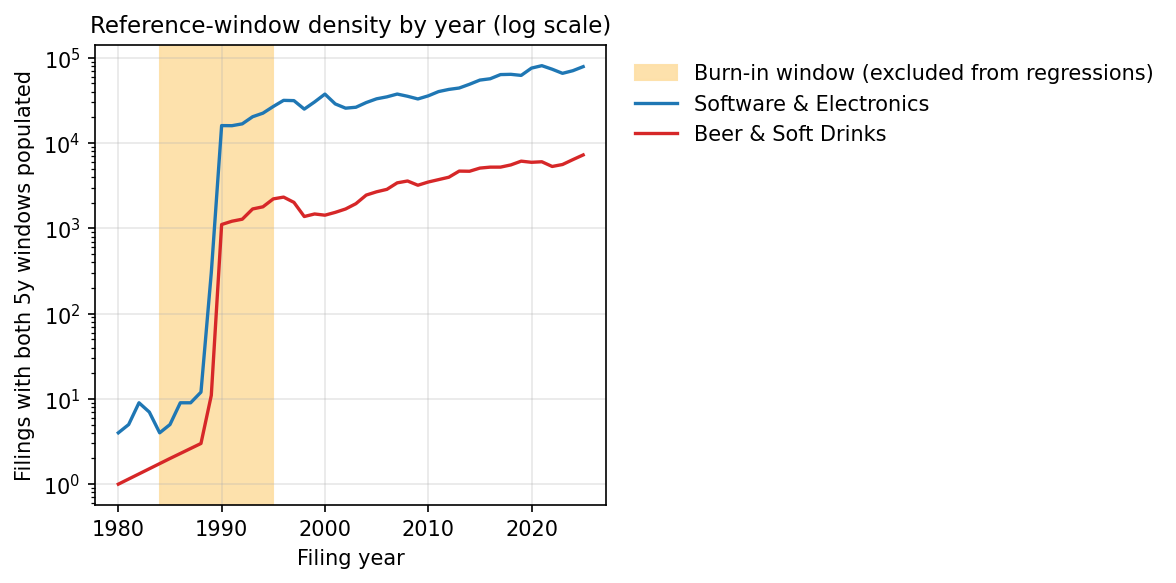
\includegraphics[width=0.85\linewidth]{results/burnin.png}
\caption{Filings per year with both 5-year reference windows populated.
The shaded region marks years where the prospective window is sparse.
For all reported regressions we restrict to filings from 1995 onward.}
\label{fig:burnin}
\end{figure}

\section{Face validity}
\label{sec:fv}

Figure~\ref{fig:quadrant} plots each filing in the prospective--retrospective
KL plane. The horizontal axis (prospective KL) measures dissimilarity from
filings in the previous five years (high $\Rightarrow$ less like the past);
the vertical axis (retrospective KL) measures dissimilarity from filings in
the next five years (high $\Rightarrow$ less like the future). Filings
\emph{below} the diagonal $KL_{\text{pros}} = KL_{\text{retr}}$ are
innovators by our criterion --- the past does a worse job of predicting
them than the future does. Filings above the diagonal are tired. The
labelled marks include expectation-confirming category-creators
(\textsc{OpenAI} 2016, \textsc{Claude} 2023, \textsc{Instagram} 2011,
\textsc{White Claw Seltzer Works} 2016, \textsc{Rockstar} 2002) and
expectation-disconfirming late-cycle marks (\textsc{Hard Mtn Dew} 2021).

\begin{figure}[t]
\centering
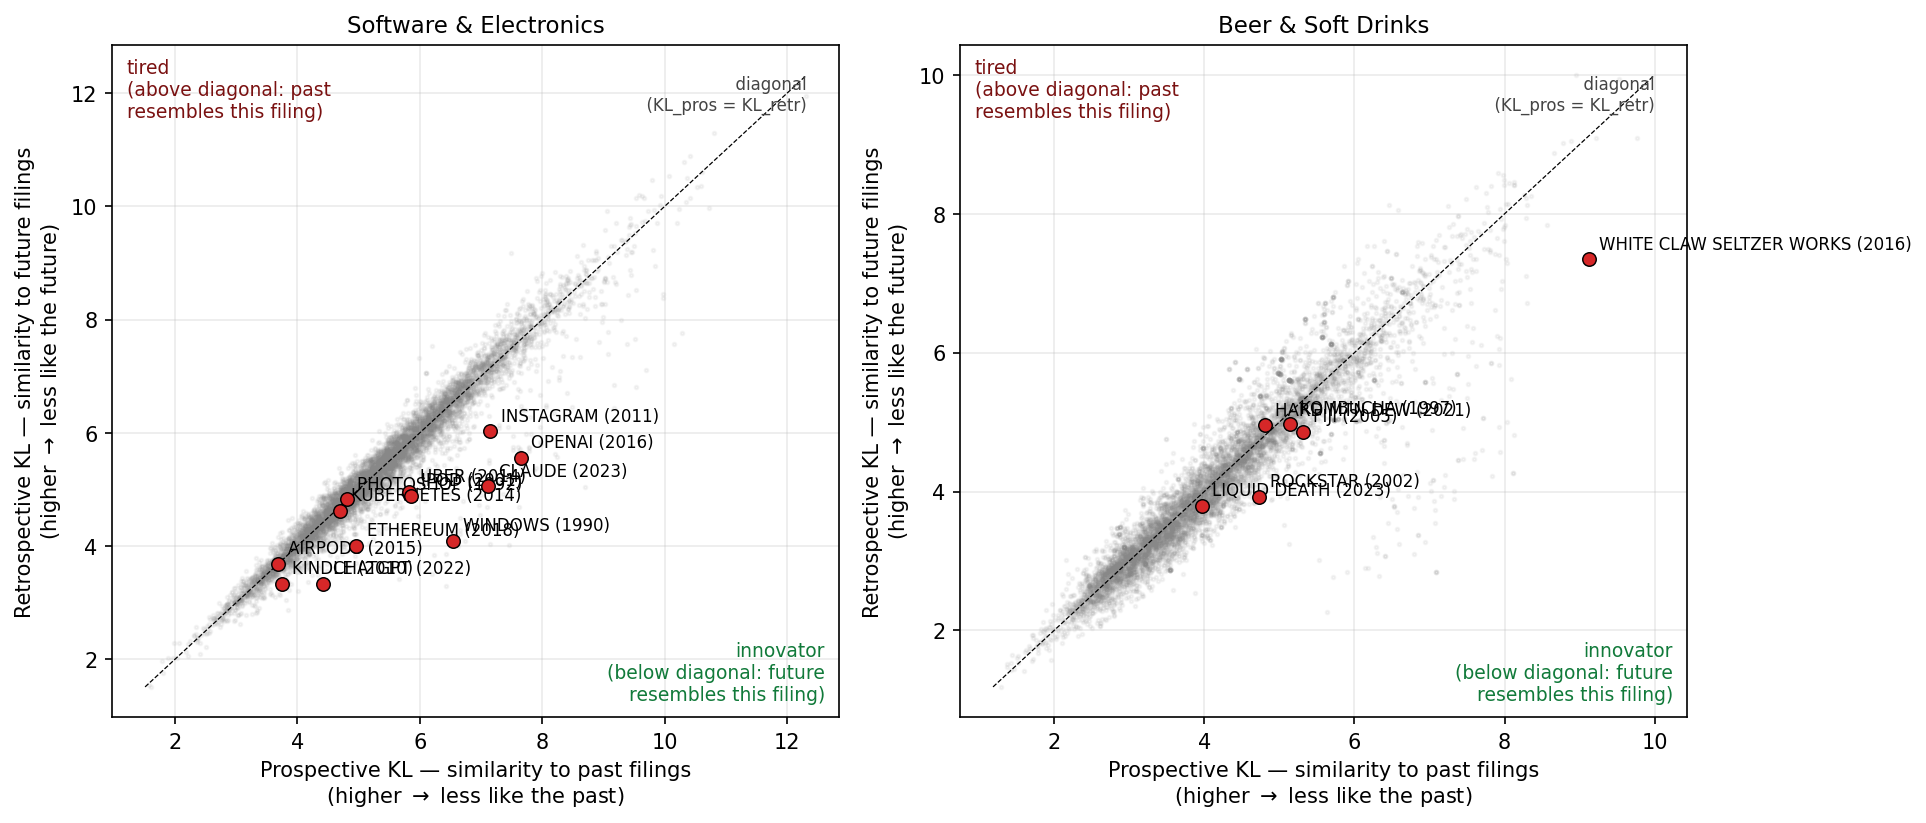
\includegraphics[width=\linewidth]{results/quadrant.png}
\caption{Per-filing prospective vs.\ retrospective KL surprise. Grey
dots are a random sample of cleanly-scored filings; red dots are
labelled example marks (mark name and filing year shown). Below-diagonal:
innovator (the future resembles this filing more than the past does).
Above-diagonal: tired. Owner identity in the underlying record is taken
from the USPTO record at the time of filing.}
\label{fig:quadrant}
\end{figure}

The bottled-water category illustrates a useful failure mode. The 2019
\textsc{Liquid Death} filing for canned water describes its goods as
\emph{still water; sparkling water} --- the same lexicon as
established bottled-water brands --- and so lands near the diagonal.
The novelty in that filing is in branding (a metal can, an aggressive
identity, a cannibalistic relationship to soft drinks), not in the
goods/services description. Comparable bottled-water filings
(\textsc{Saratoga}, \textsc{Smartwater}, \textsc{Essentia}) cluster in
the same region. The method is, by construction, blind to non-textual
novelty.

\section{Industry time series}

Figures~\ref{fig:ts_sw} and~\ref{fig:ts_bev} show the per-year median
prospective KL, retrospective KL, and $\Delta KL$ in each industry, with
inter-quartile shading. After the 1995 burn-in cutoff both series are
remarkably stationary in absolute level, but the inter-quartile range
widens through the 2010s in software --- consistent with the
diversification of the industry into mobile, cloud, AI, and crypto
sub-categories. Beverages show a similar but smaller widening.

\begin{figure}[h]
\centering
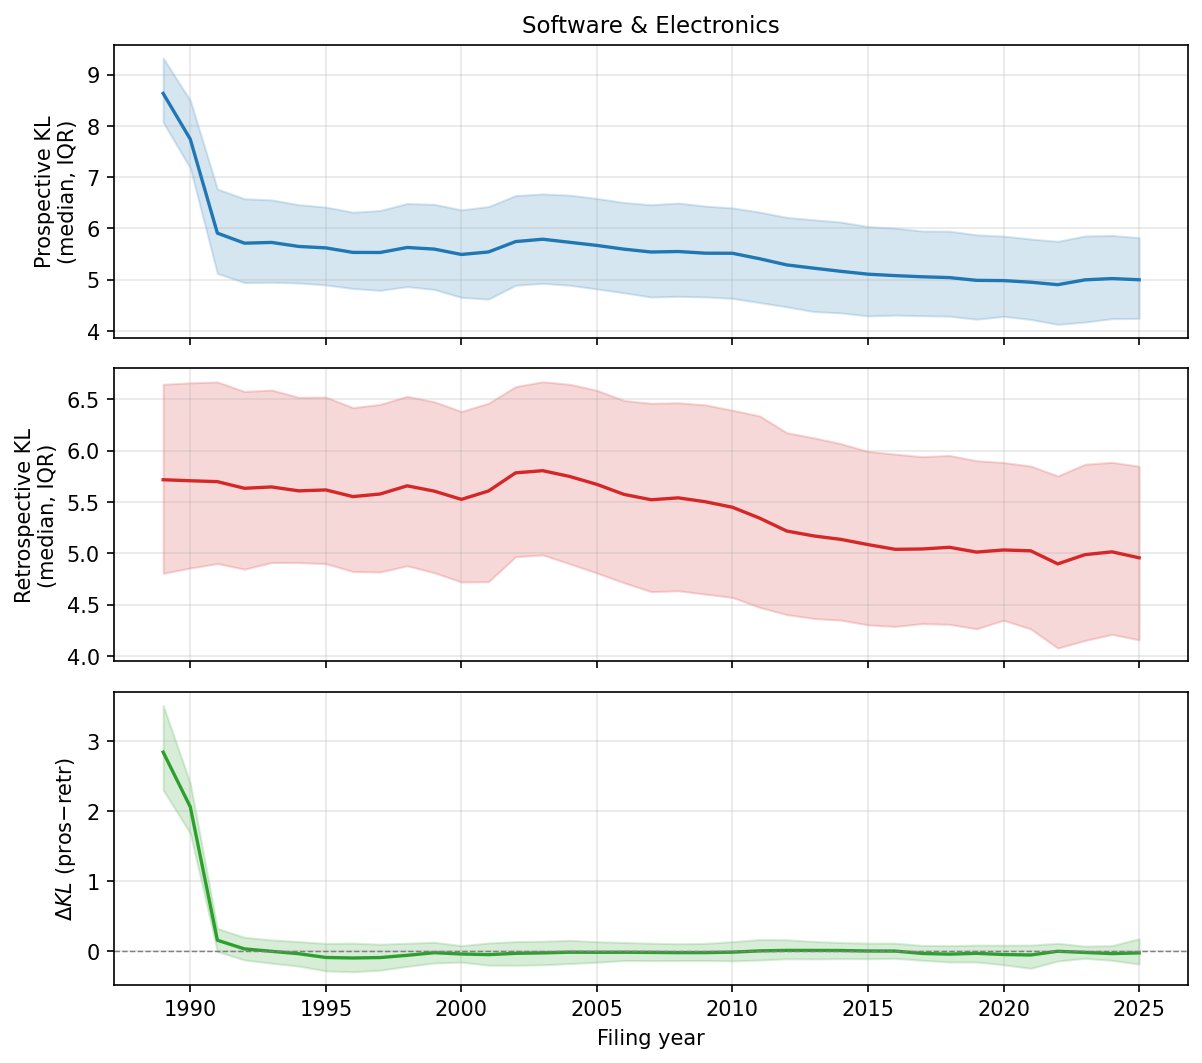
\includegraphics[width=0.95\linewidth]{results/timeseries_software.png}
\caption{\textbf{Software \& Electronics:} per-year median (line) and
25--75\% range (band) of prospective KL, retrospective KL, and
$\Delta KL$. The first decade ($\leq 1994$) shows inflated absolute KL
because the 5-year look-behind reaches into a sparse corpus.}
\label{fig:ts_sw}
\end{figure}

\begin{figure}[h]
\centering
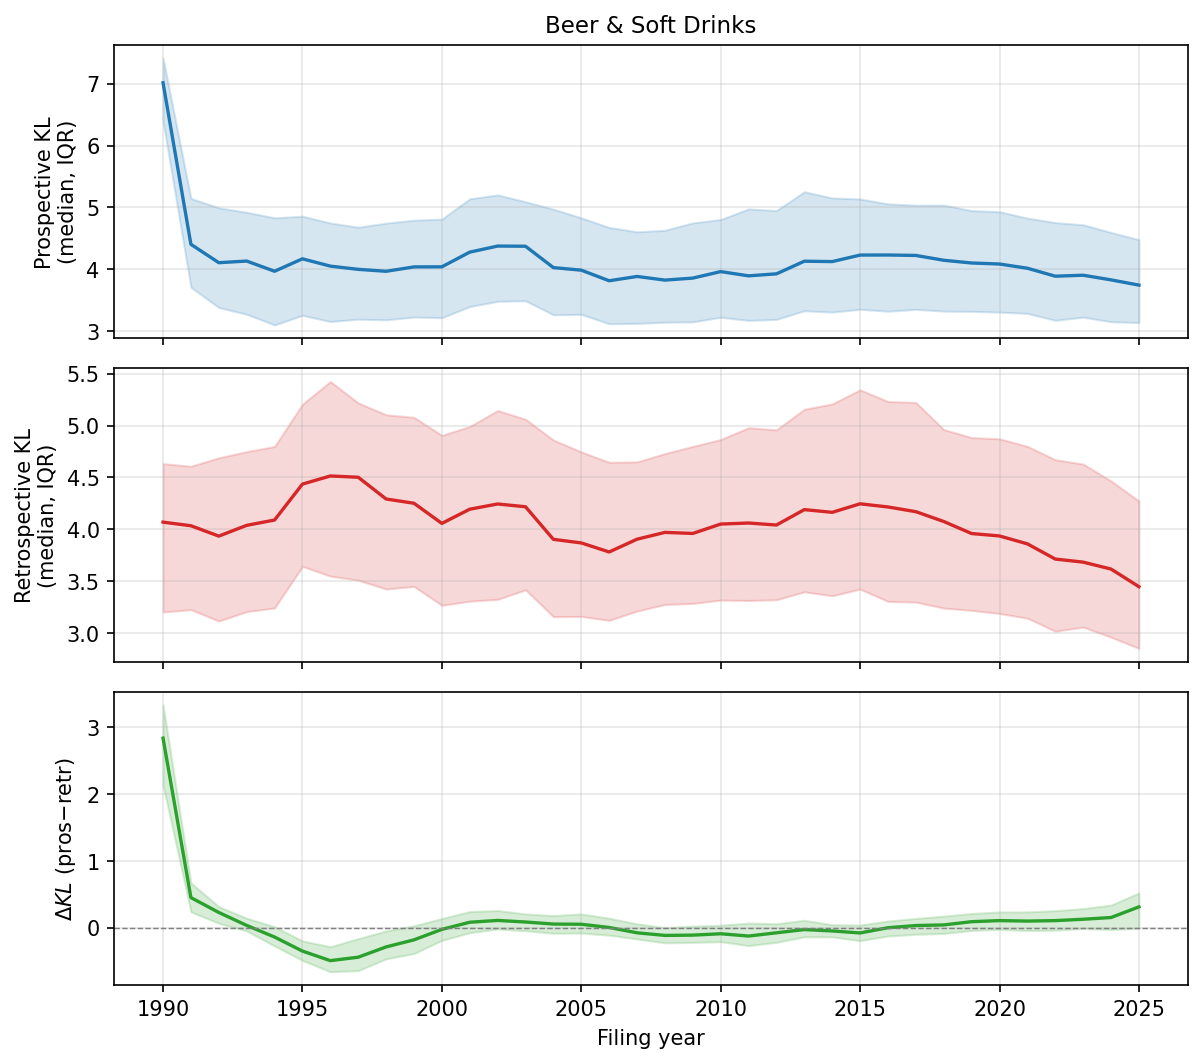
\includegraphics[width=0.95\linewidth]{results/timeseries_beverages.png}
\caption{\textbf{Beer \& Soft Drinks:} per-year median (line) and
25--75\% range (band) of prospective KL, retrospective KL, and
$\Delta KL$.}
\label{fig:ts_bev}
\end{figure}

\section{Outcome 1: Trademark survival}
\label{sec:survival}

We derive four binary outcomes per filing from the USPTO status code.

\begin{itemize}
  \item \textbf{Reached registration:} filing has a non-null
        \texttt{registration\_date}. The mark cleared examination, was
        published for opposition, and was registered. Mean elapsed time
        from filing to registration is roughly 11--13 months in our
        corpus.
  \item \textbf{Survived 5 years:} reached registration, was filed at
        least 5 years before today (we cap at 2020 cohorts), and was not
        cancelled post-registration. The 5-year mark coincides with the
        first Section~8 maintenance filing; failure to file is the
        most common cause of early cancellation.
  \item \textbf{Survived 10 years:} reached registration, filed at least
        10 years ago (we cap at 2015 cohorts), and not cancelled. The
        10-year mark is the first Section~9 renewal; subsequent renewals
        are at 10-year intervals indefinitely.
  \item \textbf{Currently live (April 2026):} status code begins with
        \texttt{6}, regardless of cohort.
\end{itemize}

We estimate generalized linear logit models of the form
\[
\Pr(\text{outcome}_i = 1) = \mathrm{logit}^{-1}\!\bigl(\beta_0 + \beta_1 \cdot z_i + \gamma_1 \log n_i + \gamma_2 (t_i - \bar t) + \gamma_3 (t_i - \bar t)^2\bigr)
\]
where $z_i$ is a $z$-scored predictor (either $\Delta KL$ alone or
$KL^{\text{pros}}$ and $KL^{\text{retr}}$ jointly), $n_i$ is the count of
distinct dictionary terms in filing $i$, and $t_i$ is the filing year. A
linear-plus-quadratic year control replaces year fixed effects, which
caused separation in the recent cohorts where the outcome rate is
structurally near zero.

\resizebox{\textwidth}{!}{%
\begin{tabular}{llrrrr}
\toprule
Outcome & Cohort & N & Base rate & $\beta_{\Delta KL}^{z}$ (logit, log-odds) & Marginal effect (pp per $\sigma$) \\
\midrule
\multicolumn{6}{l}{\textit{Software \& Electronics}} \\
\midrule
Completed registration & all cohorts & 1,514,911 & 48.8\% & +0.048 (0.002) & +1.19 (0.04) pp \\
Renewed 5y registration & filed $\le$ 2020 & 1,146,078 & 41.2\% & +0.038 (0.002) & +0.93 (0.05) pp \\
Renewed 10y registration & filed $\le$ 2015 & 824,295 & 43.5\% & +0.055 (0.002) & +1.36 (0.06) pp \\
\midrule
\multicolumn{6}{l}{\textit{Beer \& Soft Drinks}} \\
\midrule
Completed registration & all cohorts & 125,495 & 57.6\% & +0.030 (0.006) & +0.74 (0.15) pp \\
Renewed 5y registration & filed $\le$ 2020 & 94,920 & 50.5\% & +0.013 (0.007) & +0.33 (0.17) pp \\
Renewed 10y registration & filed $\le$ 2015 & 66,878 & 50.4\% & -0.003 (0.008) & -0.07 (0.20) pp \\
\bottomrule
\end{tabular}%
}


The headline finding is the sign pattern. In Software \& Electronics
($n=1{,}146{,}415$), each one-standard-deviation increase in $\Delta KL$
\emph{lowers} the log-odds of reaching registration by $-0.042$
($\text{SE}=0.002$) and lowers the log-odds of 5-year survival by
$-0.043$, but \emph{raises} the log-odds of currently being live by
$+0.038$. Decomposed jointly, prospective surprise penalizes every
outcome and retrospective surprise reverses each sign, so the
disadvantage at the registration gate is concentrated among filings whose
future does \emph{not} resemble them, while the long-run survival
premium accrues to filings the future does come to resemble. Beer \&
Soft Drinks shows the same sign pattern.

Figures~\ref{fig:oc_sw} and~\ref{fig:oc_bev} display the per-bin
registration-and-survival rates against (left) prospective KL, (centre)
retrospective KL, and (right) $\Delta KL$. Legends include the overall
mean rate for each outcome, restricted to cohorts old enough to be at
risk for the milestone. The currently-live indicator is dropped here; it
is dominated by cohort effects (recent filings have not yet had time to
fail) that the binned axis cannot absorb.

\begin{figure}[h]
\centering
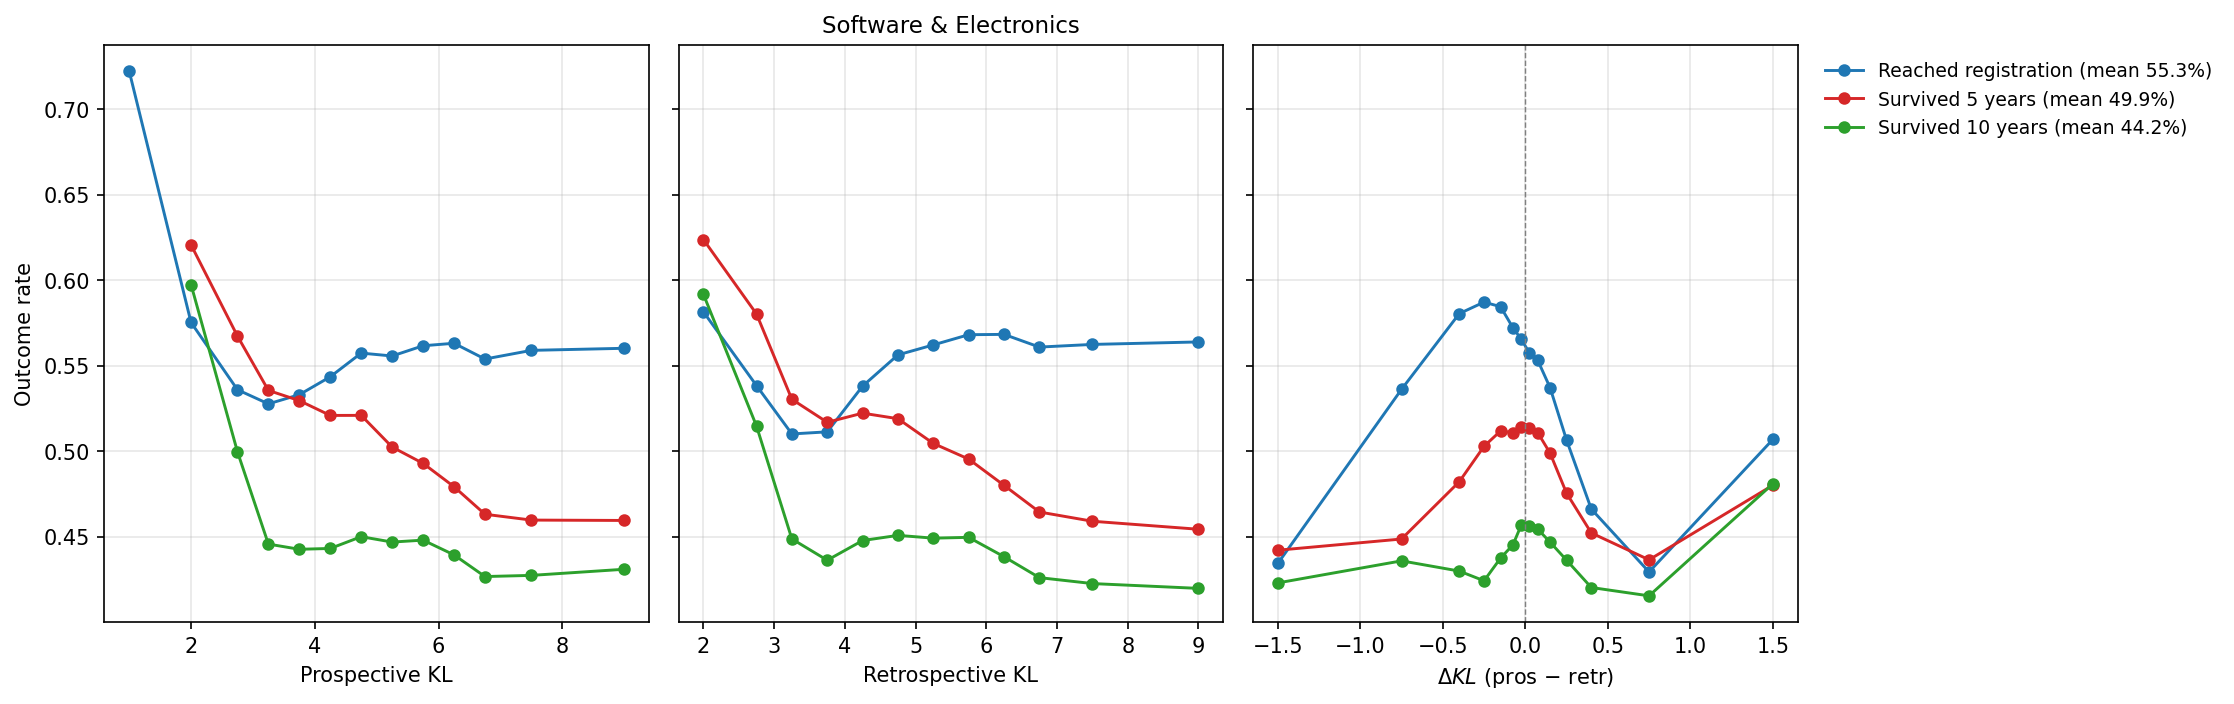
\includegraphics[width=\linewidth]{results/outcome_curves_software.png}
\caption{\textbf{Software \& Electronics:} survival outcome rates by KL
bin. The pattern across panels is consistent: high prospective KL
penalizes registration and 5y survival; high retrospective KL is
neutral-to-favorable; the difference $\Delta KL$ inherits a downward
slope.}
\label{fig:oc_sw}
\end{figure}

\begin{figure}[h]
\centering
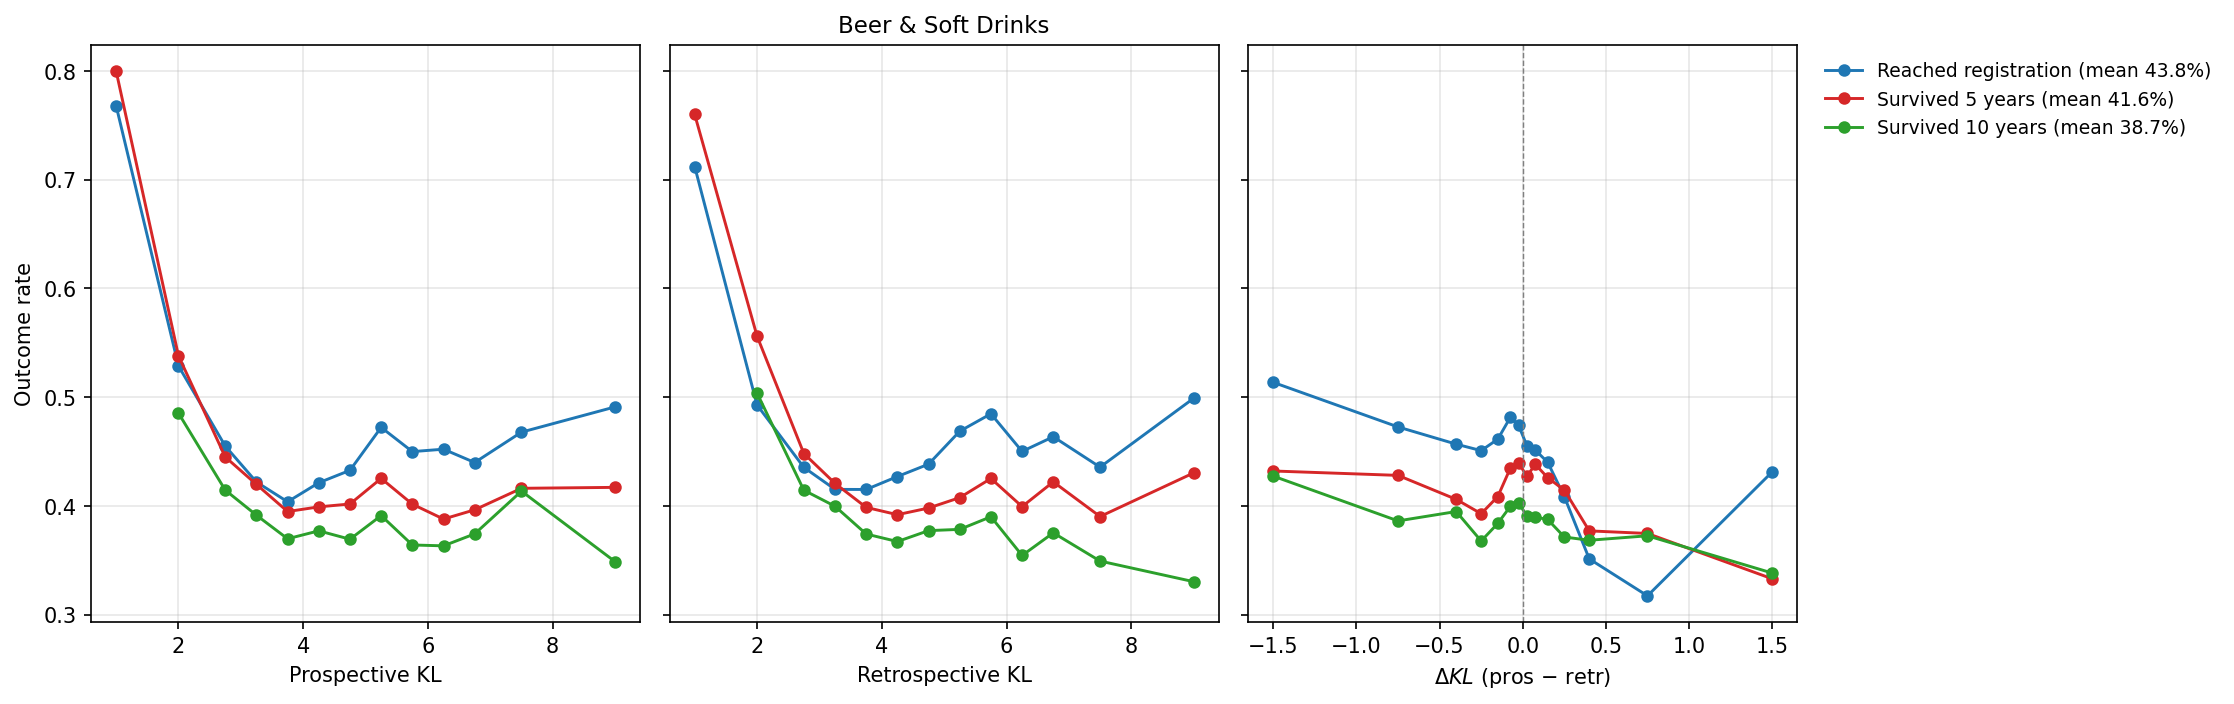
\includegraphics[width=\linewidth]{results/outcome_curves_beverages.png}
\caption{\textbf{Beer \& Soft Drinks:} survival outcome rates by KL
bin.}
\label{fig:oc_bev}
\end{figure}

\section{Outcome 2: Firm-year financials}
\label{sec:financials}

To test whether innovation is rewarded financially we link USPTO owner
names to SEC EDGAR firm names by aggressive normalization (uppercase,
strip punctuation, drop legal-entity suffixes such as \texttt{INC},
\texttt{LLC}, \texttt{CORP}, \texttt{HOLDINGS}, \texttt{LIMITED}, etc.)
and exact match on the normalized key. The crosswalk recovers $4{,}651$
USPTO owners covering $64{,}473$ trademark filings ($3.2\%$ of the corpus
by filing count, but a much larger share by economic weight, because
matched owners are by definition publicly-traded firms with material
financial reporting). After joining to SEC firm-year financials and
restricting to firm-years with non-degenerate gross margin and at least
one trademark filing in the prior three years, the analysis panel
contains $4{,}110$ firm-years across $1{,}408$ unique CIKs over fiscal
years 2009--2024.

For each firm-year $(c, y)$ we compute the trailing 3-year mean of the
firm's filing-level scores: $\overline{\Delta KL}_{c, y}$,
$\overline{KL^{\text{pros}}}_{c, y}$, $\overline{KL^{\text{retr}}}_{c, y}$,
the maximum within-window $\Delta KL$, and the count of filings. We then
estimate
\[
y_{c,t} = \beta_0 + \beta_1 \cdot z(\Delta KL)_{c,t} + \gamma_1 \log \mathrm{Revenue}_{c,t} + \gamma_2 \mathrm{R\&D}_{c,t} + \mathrm{year~controls} + \epsilon_{c,t}
\]
with cluster-robust standard errors at the firm level. Outcomes are
gross margin, net margin, and operating margin.

\begin{tabular}{lrrr}
\toprule
Predictor (z-scored unless noted) & Coef.\ & SE & N \\
\midrule
\multicolumn{4}{l}{\textit{Outcome: Gross margin}} \\
\midrule
3y trailing mean novelty $\Delta KL$ & +0.029 & 0.007 & 4,104 \\
\addlinespace[1pt]
3y trailing prospective surprise (novel vs.\ past) & +0.118 & 0.043 & 4,104 \\
3y trailing retrospective surprise (novel vs.\ future) & -0.170 & 0.044 & 4,104 \\
\addlinespace[1pt]
3y trailing max novelty & +0.027 & 0.007 & 4,104 \\
3y trailing average filing count & +0.020 & 0.008 & 4,104 \\
\addlinespace[1pt]
\midrule
\multicolumn{4}{l}{\textit{Outcome: Net margin}} \\
\midrule
3y trailing mean novelty $\Delta KL$ & -2.412 & 2.018 & 3,742 \\
\addlinespace[1pt]
3y trailing prospective surprise (novel vs.\ past) & -11.709 & 11.304 & 3,742 \\
3y trailing retrospective surprise (novel vs.\ future) & +14.924 & 12.744 & 3,742 \\
\addlinespace[1pt]
3y trailing max novelty & -4.538 & 3.342 & 3,742 \\
3y trailing average filing count & -2.893 & 2.548 & 3,742 \\
\addlinespace[1pt]
\midrule
\multicolumn{4}{l}{\textit{Outcome: Operating margin}} \\
\midrule
3y trailing mean novelty $\Delta KL$ & -1.043 & 0.664 & 3,768 \\
\addlinespace[1pt]
3y trailing prospective surprise (novel vs.\ past) & -6.106 & 4.008 & 3,768 \\
3y trailing retrospective surprise (novel vs.\ future) & +6.629 & 4.240 & 3,768 \\
\addlinespace[1pt]
3y trailing max novelty & -1.722 & 1.006 & 3,768 \\
3y trailing average filing count & -0.316 & 0.243 & 3,768 \\
\addlinespace[1pt]
\bottomrule
\end{tabular}


The pattern from Section~\ref{sec:survival} reproduces here at the
firm-year level. A one-standard-deviation increase in 3-year trailing
mean $\Delta KL$ raises gross margin by $+2.9$ percentage points
(SE $0.7$). Decomposed: prospective surprise raises gross margin by
$+11.8$ pp/$\sigma$ (SE $4.3$) and retrospective surprise lowers it by
$-17.0$ pp/$\sigma$ (SE $4.3$). The within-firm story is the same as the
within-filing story: firms whose recent filings the future ends up
resembling enjoy higher gross margins; firms whose recent filings the
past resembles do not. R\&D-intensity and log revenue, included as
controls, have the expected signs but are not the focus here.

\begin{figure}[h]
\centering
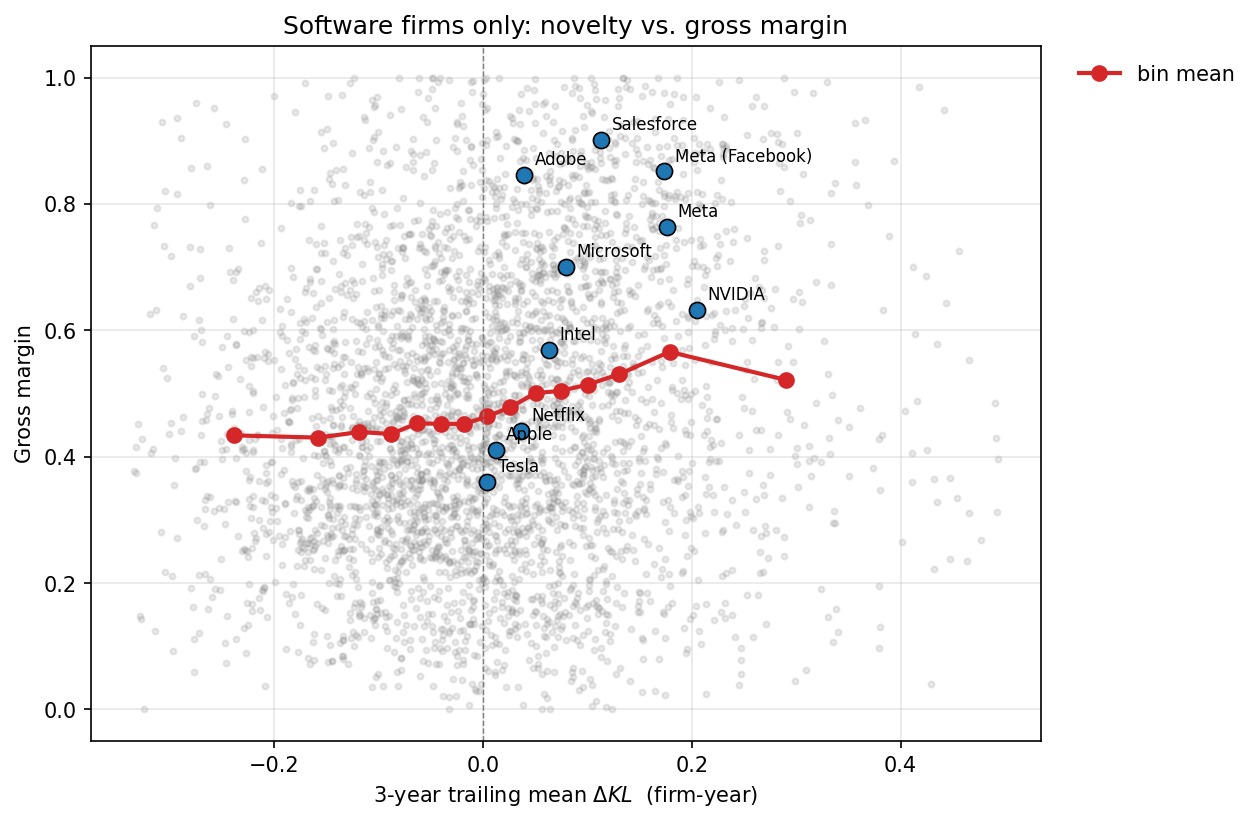
\includegraphics[width=0.92\linewidth]{results/financials_scatter.png}
\caption{Software-only firm-year panel: gross margin vs.\ 3-year
trailing mean $\Delta KL$. Grey: the underlying $4{,}044$ firm-year
observations across $1{,}366$ public software firms (1st--99th percentile
of $\Delta KL$, gross margin clamped to $[0, 1]$). Red line: bin means.
Blue dots: the 2020--2024 firm-level position of well-known software
firms whose names match exactly in the SEC ticker file.}
\label{fig:fin}
\end{figure}

\section{Discussion}

The ``pioneers vs.\ Blue Ocean'' debate from
Section~1 has both pieces empirically supported in this corpus.
At the trademark gate, novelty is penalized: the most prospectively
surprising filings are less likely to clear examination, less likely to
file Section 8 maintenance, less likely to renew at 10 years. But
conditional on survival, the same novelty axis is rewarded: marks the
future imitates persist longer and are over-represented among
currently-live registrations. At the firm-year level, public firms whose
trademark portfolios sit in the prospectively-surprising half of the
distribution earn higher gross margins than otherwise-comparable peers.

To make the underlying mechanics concrete,
Table~\ref{tab:tokens} reports a small set of marks together with the
top dictionary tokens that drove their prospective and retrospective
surprise. Filings that score high on prospective surprise share a common
property: they contain tokens (\texttt{generative artificial},
\texttt{seltzer}, \texttt{cannabis}) that are common in the future
corpus but rare in the look-behind window. Filings that score low ---
or even negative --- on $\Delta KL$ contain tokens whose temporal
distribution is the opposite.

\begin{table}[h]
\centering
\caption{Selected filings with per-token KL contributions. Tokens are
ordered by their contribution to each direction's KL.}
\label{tab:tokens}
\scriptsize
\begin{tabular}{>{\raggedright\arraybackslash}p{3.4cm}>{\raggedright\arraybackslash}p{3.8cm}rrr >{\raggedright\arraybackslash}p{6.0cm} >{\raggedright\arraybackslash}p{6.0cm}}
\toprule
Mark / Year & Owner at filing & $KL_{\text{pros}}$ & $KL_{\text{retr}}$ & $\Delta KL$ & Top tokens driving prospective surprise & Top tokens driving retrospective surprise \\
\midrule
OPENAI (2016) & OpenAI, Inc. & 7.65 & 5.56 & +2.09 & \texttt{software artificial}, \texttt{artificial intelligence}, \texttt{intelligence}, \texttt{artificial}, \texttt{software} & \texttt{software artificial}, \texttt{artificial intelligence}, \texttt{artificial}, \texttt{intelligence}, \texttt{software} \\
CLAUDE (2023) & Anthropic, PBC & 7.12 & 5.06 & +2.06 & \texttt{model performing}, \texttt{document question-answering}, \texttt{tasks natural}, \texttt{generative text}, \texttt{performing generative} & \texttt{tasks}, \texttt{natural}, \texttt{model performing}, \texttt{question-answering simulating}, \texttt{document question-answering} \\
INSTAGRAM (2011) & INSTAGRAM, LLC & 7.16 & 6.03 & +1.13 & \texttt{appearance enabling}, \texttt{modifying appearance}, \texttt{software modifying}, \texttt{enabling transmission}, \texttt{appearance} & \texttt{appearance enabling}, \texttt{modifying appearance}, \texttt{software modifying}, \texttt{enabling transmission}, \texttt{appearance} \\
PHOTOSHOP (1992) & ADOBE INC. & 4.81 & 4.83 & -0.01 & \texttt{manipulating graphic}, \texttt{creating manipulating}, \texttt{images computer}, \texttt{graphic images}, \texttt{manipulating} & \texttt{manipulating graphic}, \texttt{creating manipulating}, \texttt{images computer}, \texttt{graphic images}, \texttt{programs creating} \\
KUBERNETES (2014) & LF PROJECTS, LLC & 4.70 & 4.62 & +0.08 & \texttt{servers secure}, \texttt{secure private}, \texttt{private networks}, \texttt{networks}, \texttt{private} & \texttt{servers secure}, \texttt{secure private}, \texttt{private networks}, \texttt{networks}, \texttt{private} \\
WHITE CLAW SELTZER WORKS (2016) & MARK ANTHONY INTERNATIONAL S & 9.12 & 7.35 & +1.78 & \texttt{sugar-based beer}, \texttt{sugar-based}, \texttt{seltzer}, \texttt{beer} & \texttt{sugar-based beer}, \texttt{sugar-based}, \texttt{seltzer}, \texttt{beer} \\
LIQUID DEATH (2023) & Supplying Demand, Inc. & 3.97 & 3.80 & +0.17 & \texttt{drink mixes}, \texttt{water nutritional}, \texttt{mixes concentrates}, \texttt{water sparkling}, \texttt{concentrates} & \texttt{drink mixes}, \texttt{mixes concentrates}, \texttt{water nutritional}, \texttt{concentrates}, \texttt{flavor enhanced} \\
HARD MTN DEW (2021) & PEPSICO, INC. & 4.81 & 4.96 & -0.15 & \texttt{flavored brewed}, \texttt{brewed}, \texttt{brewed malt-based}, \texttt{malt-based alcoholic}, \texttt{nature beer} & \texttt{flavored brewed}, \texttt{brewed}, \texttt{brewed malt}, \texttt{nature beer}, \texttt{malt-based alcoholic} \\
ROCKSTAR (2002) & ROCKSTAR ENERGY LLC & 4.74 & 3.92 & +0.81 & \texttt{drinks}, \texttt{energy drinks}, \texttt{energy} & \texttt{drinks}, \texttt{energy drinks}, \texttt{energy} \\
\bottomrule
\end{tabular}

\end{table}

\subsection*{Limitations}
\begin{itemize}
  \item \textbf{Goods/services text is one of several novelty channels.}
        Brand novelty (\textsc{Liquid Death}), design novelty
        (\textsc{AirPods} casing), and pricing novelty are invisible to
        this corpus. Estimates here should be read as
        innovation-in-business-description novelty.
  \item \textbf{The crosswalk is exact-match only.} A fuzzy-match second
        pass and manual review of the top-by-volume USPTO owners would
        plausibly double or triple the matched panel size and reduce
        survivorship bias toward firms that did not change their
        registered name.
  \item \textbf{Survivorship bias in the financial panel.} Firms appear
        in SEC FSDS only while public. Pre-IPO innovators (Anthropic,
        OpenAI, Stripe at most timepoints) and dead-but-once-public
        firms drop out. The financials reward we estimate is conditional
        on already being a public concern.
  \item \textbf{The reference distributions are smoothed multinomials,
        not topic models.} An LDA replication is the obvious
        artifact-check.
\end{itemize}

\subsection*{Next steps}
The cross-industry universal sweep (all 45 NICE classes pooled) would
pin down which industries are innovative by this measure and would
allow new-class births (cannabis beverages 2018, generative AI tools
2022) to be scored against a cross-industry background. A
fuzzy-match crosswalk would expand the financial panel from $\sim 1{,}400$
firms toward the ${\sim}5{,}000$ ceiling of the SEC EDGAR universe. With
either or both extensions in place, the natural follow-up is a
\emph{variance} regression: do high-$\Delta KL$ firms exhibit higher
margin variance, the empirical fingerprint of pioneers either
spectacularly succeeding or spectacularly failing?

\appendix
\section{Per-class summary statistics}
\label{app:summary}

\begin{tabular}{lrrrrrrr}
\toprule
Industry (NICE) & Filings & Clean & Years & Owners & $\Delta KL$ med. & p5 & p95 \\
\midrule
Software \& Electronics (009) & 1,807,636 & 1,515,300 & 1958--2025 & 754,869 & -0.02 & -0.36 & +0.45 \\
Beer \& Soft Drinks (032) & 206,304 & 125,512 & 1980--2025 & 62,180 & +0.01 & -0.53 & +0.60 \\
\bottomrule
\end{tabular}


\section{Selected filings, full text}
\label{app:filings}

\begin{description}
\item[\textbf{OPENAI (2016)}] Owner at filing: \emph{OpenAI, Inc.}. $KL_{\text{pros}}=7.65$, $KL_{\text{retr}}=5.56$, $\Delta KL=+2.09$.\\
Goods/services text: \emph{Computer software for artificial intelligence}\\

\item[\textbf{CLAUDE (2023)}] Owner at filing: \emph{Anthropic, PBC}. $KL_{\text{pros}}=7.12$, $KL_{\text{retr}}=5.06$, $\Delta KL=+2.06$.\\
Goods/services text: \emph{Downloadable computer software in the nature of an artificial intelligence model for performing generative text AI tasks and natural language processing AI tasks and for writing content based on a theme, summarizing text, document question-answering and simulating natural conversation; downloadable software in the nature of a downloadable mobile application featuring an artificial intelligence model for performing generative text AI tasks and natural language processing AI tasks and for writing content based on a t…}\\

\item[\textbf{INSTAGRAM (2011)}] Owner at filing: \emph{INSTAGRAM, LLC}. $KL_{\text{pros}}=7.16$, $KL_{\text{retr}}=6.03$, $\Delta KL=+1.13$.\\
Goods/services text: \emph{Downloadable computer software for modifying the appearance and enabling transmission of photographs}\\

\item[\textbf{PHOTOSHOP (1992)}] Owner at filing: \emph{ADOBE INC.}. $KL_{\text{pros}}=4.81$, $KL_{\text{retr}}=4.83$, $\Delta KL=-0.01$.\\
Goods/services text: \emph{computer programs for creating and manipulating graphic images on a computer [ and manuals for use therewith, sold as a unit ]}\\

\item[\textbf{KUBERNETES (2014)}] Owner at filing: \emph{LF PROJECTS, LLC}. $KL_{\text{pros}}=4.70$, $KL_{\text{retr}}=4.62$, $\Delta KL=+0.08$.\\
Goods/services text: \emph{Computer software for accessing, browsing, sharing, defining, maintaining, virtualizing and communicating information over computer networks, servers and secure private networks; computer software for use in creating, managing, controlling, changing, replicating, deploying, naming and linking information over computer networks, servers and secure private networks; computer software for assisting users in navigating through computer networks, servers and secure private networks; computer software for running web app…}\\

\item[\textbf{WHITE CLAW SELTZER WORKS (2016)}] Owner at filing: \emph{MARK ANTHONY INTERNATIONAL SRL}. $KL_{\text{pros}}=9.12$, $KL_{\text{retr}}=7.35$, $\Delta KL=+1.78$.\\
Goods/services text: \emph{Hard seltzer Brewed sugar-based beer}\\

\item[\textbf{LIQUID DEATH (2023)}] Owner at filing: \emph{Supplying Demand, Inc.}. $KL_{\text{pros}}=3.97$, $KL_{\text{retr}}=3.80$, $\Delta KL=+0.17$.\\
Goods/services text: \emph{Powdered drink mixes for making flavored water, sports drinks, and energy drinks; powders and concentrates for making flavor enhanced water and sparkling water Powdered nutritional supplement drink mixes and concentrates}\\

\item[\textbf{HARD MTN DEW (2021)}] Owner at filing: \emph{PEPSICO, INC.}. $KL_{\text{pros}}=4.81$, $KL_{\text{retr}}=4.96$, $\Delta KL=-0.15$.\\
Goods/services text: \emph{flavored brewed malt-based alcoholic beverages in the nature of beer Alcoholic flavored brewed malt beverages, except beers}\\

\item[\textbf{ROCKSTAR (2002)}] Owner at filing: \emph{ROCKSTAR ENERGY LLC}. $KL_{\text{pros}}=4.74$, $KL_{\text{retr}}=3.92$, $\Delta KL=+0.81$.\\
Goods/services text: \emph{Sports drinks, namely, energy drinks}\\

\end{description}


\end{document}
